% 2006 上海卷文科 Q13；只保留原图中的平行四边形轮廓与四个顶点标签。
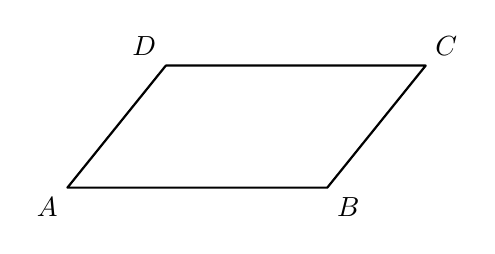
\begin{tikzpicture}[line cap=round,line join=round]
  \coordinate (A) at (0,0);
  \coordinate (B) at (3.3,0);
  \coordinate (C) at (4.55,1.55);
  \coordinate (D) at (1.25,1.55);

  \draw[thick] (A)--(B)--(C)--(D)--(A);
  \node[below left] at (A) {$A$};
  \node[below right] at (B) {$B$};
  \node[above right] at (C) {$C$};
  \node[above left] at (D) {$D$};
\end{tikzpicture}
